% !TeX spellcheck = en_US
%\documentclass[review]{cvpr}
%\documentclass[rebuttal]{cvpr}
\documentclass[final]{cvpr}
\usepackage[utf8]{inputenc}
\usepackage[backend=bibtex]{biblatex}
\bibliography{report}
\usepackage{array}
% insert graphics
\usepackage{graphicx}
\usepackage{hyperref}
% keep floats in appendix
\usepackage{float}
% pseudocode algorithms
\usepackage{algorithm}
\usepackage[noend]{algpseudocode}
\renewcommand{\algorithmicrequire}{\textbf{Input:}}

\newcommand{\algorithmautorefname}{Algorithm}
\renewcommand{\subsectionautorefname}{\sectionautorefname}
\renewcommand{\subsubsectionautorefname}{\sectionautorefname}

\title{Project Report for Machine Learning in Cyber Security:\\
\large Adversarial attacks on an LSTM malware detector}
\author{The Hidden Adversaries (Tomas Amado, Deepanshu Mehta, Marco Schuster)}
%TODO adversarial attacks -> evasion attacks?

\begin{document}

\maketitle

\section*{Abstract}
Potentially devastating malware gets increasingly detected using machine 
learning (ML) techniques. Most promisingly this is done using the malware's 
dynamic behavior such as sequences of operating system API calls. However, 
these detection/classification techniques are highly vulnerable to targeted 
modifications of the malware to 
classify it as benign. In this report we investigate such an attack and compare 
its effectiveness between viewing the malware classifier as a white-box and a 
black-box model. We observe that the attack is more than 98\% effective 
regardless of this setting. Moreover, we show that on average it requires less 
than 18\% adversarially added API calls to classify malware as benign. 
Subsequently, we show that training a malware classifier with adversarial 
samples as a defense method has a low impact on its performance while being 
highly effective against attacks. In numbers, this attack effectiveness was 
reduced from more than 98\% to less than 1\%.

\section{Introduction}
In an increasingly digitalized world the presence of malware and the damages 
caused by it became and remain a significant problem. As shown in a 2020 
Malwarebytes report \autocite[6]{malware20} the presence of malware especially 
increased in businesses. Furthermore, the possibly severe damages were recently 
illustrated by NotPetya in June 2017 taking down several international 
organizations \autocite{petya}. To tackle this threat there has been an 
increasing focus in research \autocite{agrawal2018robust, Han19, 
DBLP:journals/corr/Kim2018, DBLP:journals/corr/Lu2019} to 
detect malware with machine learning (ML) techniques 
due to their automatic training and generalization capabilities 
\autocite[1]{DBLP:journals/corr/RosenbergSRE17}. This detection can be divided 
into static analysis where typically the source, assembly or binary code of a 
program is evaluated and dynamic analysis where a programs behavior during 
execution is observed \autocite[209]{Han19}. Naturally, these ML detection 
techniques become part of the attack surface as well and an attacker might try 
to purposefully compose malware that remains undetected by a ML method.

Our research presented in this report focuses on malware classification using 
dynamic analysis for the Windows operating system. For this a publicly 
available dataset was used, a ML 
classifier was trained, this classifier was attacked in a black-box and 
white-box scenario and the classifier was defended against these attacks 
through adversarial training. The following sections present a brief overview 
over the necessary theoretical background (\autoref{sec:background}), explain 
our experimental setting (\autoref{sec:setting}), 
present and discuss our results (\autoref{sec:results}) and finally draw a 
conclusion (\autoref{sec:conclusion}).
\section{Background}
\label{sec:background}
\textit{Long Short-Term Memory (LSTM)} networks are a special type of recurrent 
neural networks used to process sequences of inputs. They are memory-based 
meaning that they store some condensed information (cell state) in between each 
sequence step. In particular, LSTM networks are popular since they fix the 
issue of vanishing and exploding gradients that regular recurrent neural 
network have and effectively capture long-term dependencies. 
\autocite[3]{agrawal2018robust} \autocite[1]{DBLP:journals/corr/GreffSKSS15}

\textit{Pooling layers} are used in neural networks to down-sample an input 
(e.g. image or sequence) to summarize its features. This is either done by 
averaging over a certain dimension and range of the input or by taking the 
maximum value of that range in that dimension. This generally makes the neural 
network more robust against translations and reduces the computational effort. 
\autocite{pooling19}

\textit{Adversarial attacks} are attacks on ML models that vary input samples 
very slightly but in such a targeted way that the model misclassifies that 
sample. Such attacks can be divided into white-box attacks where all details of 
the model (architecture, weights etc.) are known to the attacker and black-box 
attacks where these details remain hidden and only the model output can be 
observed by the attacker. \autocite[186]{voynov20}

% binary cross entropy loss???
% early stopping???
% one-hot encoding???

\section{Experimental setting}
\label{sec:setting}
\subsection{Dataset}
For the experiments conducted in this project the publicly available Windows 
API Call sequence dataset \autocite{tqqm-aq14-19} with 43,876 samples was used. 
Of these samples there are 42,797 malware and 1,079 goodware samples which are 
labeled accordingly (malware = 1, goodware = 0). Each sample is represented by 
a sequence of the first 100 consecutive and non-repeated API calls that were 
performed by the software. Each sequence element represents a particular API 
function that was called but disregards the function parameters and return 
values. In total there exist 264 distinct API functions in the dataset. 
\autocite{tqqm-aq14-19}

In order to classify this dataset with a ML model each sequence element was 
represented by a one-hot encoded vector. Moreover, the sequence length was 
extended from 100 to 150 where zero vectors were padded at the end. This was 
necessary to facilitate the attacks performed later. Finally, the samples were 
randomly split into 
training, test and validation set with 35,100 (80\%), 4,388 (10\%) and 4,388 
(10\%) samples respectively. This was performed in a stratified fashion i.e. 
retaining the original proportion of class labels in each set.
\subsection{LSTM malware classifier}
\subsubsection{Architecture}
In order to perform attacks on a malware classifier, this classifier had to be 
built and trained. As shown in \autoref{fig:lstm-architecture} we chose an 
architecture that combines LSTM cells with Max Pooling as in 
\autocite[4]{agrawal2018robust}. A very similar architecture 
with average pooling can also be found in \autocite[4]{papernot2016crafting}. 
In this initial architecture we have a single LSTM layer that processes the 
sequence of one-hot encoded API calls $x$ and outputs a sequence of 
hidden state vectors $h$. Each of these API calls and hidden state vectors is 
denoted as $x[t]$ and $h[t]$ respectively. Subsequently, a one dimensional 
pooling over all $h[t]$ is 
performed and finally a fully connected layer with sigmoid activation function 
outputs the probability of the input being malicious. The size of the hidden 
state vector was initially picked as $h_{LSTM} = 128$ as in 
\autocite[10]{DBLP:journals/corr/RosenbergSRE17}.
\begin{figure}
	\centering
	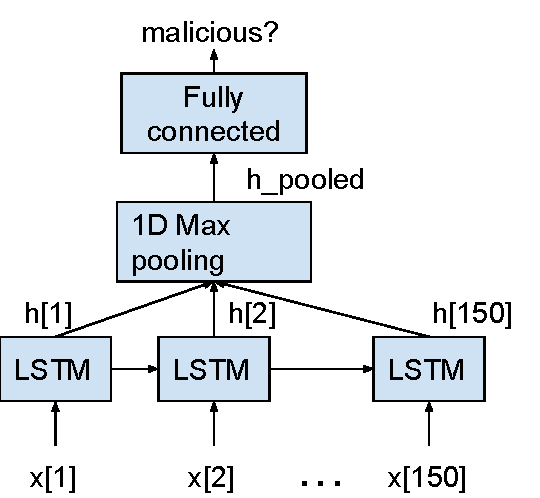
\includegraphics[width=5cm]{lstm-architecture}
	\caption{Architecture of LSTM malware classifier}
	\label{fig:lstm-architecture}
\end{figure}
\subsubsection{Training and tuning}
\label{sec:train}
All training of this classifier was performed with an Adam optimizer 
\autocite{kingma2017adam} with default parameters and a batch size of 256 
samples. Furthermore, an early stopping implementation \autocite{Sunde20} with 
a patience of 7 epochs was used as a regularization method. As a loss we chose 
a binary cross entropy loss since we have a binary classification problem. 
Also, the loss was weighted by the relative frequency of classes in the 
dataset. This was necessary since equal weights for both classes lead to a very 
imbalanced performance of the classifier (validation sensitivity 99.9\%, 
validation specificity 61.1\%) due to the significant class imbalance in the 
dataset.

To get a reasonably good classifier to attack, different hyper-parameters of 
the architecture were tuned individually. These were the type of pooling layer 
$pool \in \{max, avg\}$, the number of LSTM layers $l_{LSTM}$ and the size of 
the hidden state vector $h_{LSTM}$. The details of this tuning are shown in the 
appendix in \autoref{tab:architecture-tuning}. The best model in terms of 
validation loss used $l_{LSTM} = 1$, $h_{LSTM} = 128$ and 
$pool = max$ which we then evaluated on the test set. The results were a test 
sensitivity (accuracy on malware) of 97.6\% and a test specificity (accuracy on 
goodware) of 93.5\%. These are similar to or slightly below the accuracies 
achieved in \autocite[11]{DBLP:journals/corr/RosenbergSRE17} and 
\autocite[7]{agrawal2018robust} and thus a reasonably good classifier was 
obtained.

\subsection{Black-box attack}
\subsubsection{Surrogate model training}
\label{sec:surrogate-model-training}
Since no detailed information about the attacked model is available in the 
black-box setting, a surrogate model with preferably very similar behavior had 
to be trained. This was performed with a variant of Jacobian-based dataset 
augmentation as presented in \autocite[5-6]{DBLP:journals/corr/RosenbergSRE17}. 
The procedure for this is shown in \autoref{alg:surrogate-model}.

\begin{algorithm}
	\caption{Surrogate model training inspired by 
	\autocite[6]{DBLP:journals/corr/RosenbergSRE17}}
	\label{alg:surrogate-model}
	\begin{algorithmic}[1]
		\Require $f$ (black-box model), $\hat{f}$ (surrogate model), $T_a$ 
		(augmentation epochs), $T_b$ (training epochs), $X_1$ (initial 
		dataset), $\epsilon$ (perturbation factor)
		\For{$k=1..T_a$}
			\State $y_k \gets \{f(x) | x \in X_k\}$
			\State train($\hat{f}$, $X_k$, $y_k$, $T_b$)
			\If {$k \neq T_a$}
				\State $X_{k+1} \gets \{x + \epsilon \cdot sign(J_{\hat{f}}[x]) 
				| x \in X_k\} \cup X_k$
			\EndIf
		\EndFor
	\end{algorithmic}
\end{algorithm}

Basically, the attacker trains the surrogate model using the output 
probabilities of the 
black-box model $y_k$ (lines 2 and 3). However, the attacker only has access 
to a relatively small initial dataset $X_1$ and aims to keep the number of 
queries to the black-box model low. Therefore, the dataset to query the 
black-box model with is iteratively augmented with samples where the model 
output varies the most (line 5). This is done by evaluating the sign of the 
Jacobian $sign(J_{\hat{f}}[x])$ of the surrogate model $\hat{f}$ at each sample 
$x$. \autocite[5-6]{DBLP:journals/corr/RosenbergSRE17}

Our variant of this algorithm furthermore calculates these augmentations 
only if the algorithm is not in the last iteration (line 4) since the 
augmentation is very computationally expensive and it seems wasteful to augment 
a dataset that remains unused. The \textit{train} function used the same basic 
training procedure as described in \autoref{sec:train} but without early 
stopping. Besides that, we used $T_a = 3$ augmentation 
epochs, $T_b = 10$ training epochs, the validation set as the initial dataset 
$X_1$ and a perturbation factor $\epsilon = 0.01$. Additionally, the surrogate 
model $\hat{f}$ differs architecturally from the black-box model $f$ since its 
architecture remains unknown to the attacker. The changes for $\hat{f}$ were 
$l_{LSTM} = 2$ and $h_{LSTM} = 256$.


\subsubsection{Generating adversarial samples}
To generate adversarial samples we used a variation of the adversarial 
sequence generation algorithm presented in 
\autocite[7]{DBLP:journals/corr/RosenbergSRE17} which is shown in 
\autoref{alg:sequence generation}. The algorithm takes a sequence of API calls 
$x$ that is considered malicious by the black-box model and inserts API calls 
$a$ that are already present in the dataset into random positions until the 
sequence is classified as benign. This pure insertion ensures a minimal impact 
on the malware's functionality. When a new call is added, the rest of the calls 
to its right are shifted one position into the zero-padding. The 
sequence generation is stopped if it reaches 50 API call additions to avoid 
losing any of the original API calls. The API call $a$ to 
add is picked so that the sign of the sequence change $sign(x - x[1: i-1] \perp 
api \perp x[i: 149])$ is most similar to the direction indicated by the sign of 
the Jacobian of the surrogate model $sign(J_{\hat{f}}[x])$ where $\perp$ 
denotes sequence concatenation. This procedure is necessary since the set of 
valid API calls is discrete and limited. 
\autocite[6-8]{DBLP:journals/corr/RosenbergSRE17}


\begin{algorithm}
	\caption{Adversarial sequence generation inspired by
	\autocite[7]{DBLP:journals/corr/RosenbergSRE17}}
	\label{alg:sequence generation}
	\begin{algorithmic}[1]
		\Require $f$ (black-box model),  $\hat{f}$ (surrogate model), $x$ 
		(malicious sequence to perturb, with $l$ valid API calls)
		\While {$f(x) = malicious$ \textbf{and} valid API calls in sequence $<$ 
		150}
		    \State pick random position $i$ between $1$ and $l$
			\State $a \gets {\arg\min}_{api} ||sign(x - x[1: i-1] \perp 
			api \perp x[i: 149]) - sign(J_{\hat{f}}[x])||_2$
			\State $x \gets x[1: i-1] \perp a \perp x[i: 149]$
		\EndWhile
		\Return $x$
	\end{algorithmic}
\end{algorithm}

% TODO extra subsection for random attack?
Initially, the malicious samples of the validation set were used to generate 
adversarial samples. Moreover, as a baseline to show this method's 
effectiveness, we also generated adversarial sequences picking $a$ randomly as 
well.

\subsection{White-box attack}

The white-box attack we performed is mostly the same as the black-box attack. 
The only difference ist that we used the same model $f$ for the predictions and 
the Jacobian.

\subsection{Adversarial training} 
We investigated adversarial training to defend our model against the 
aforementioned attacks. 
For this the model was re-trained from scratch using the hyper-parameters tuned 
in \autoref{sec:train}. However, this time besides the training set we also 
used the adversarial samples generated by the white-box attack. These 
adversarial samples were also randomly split into a training and validation set 
with 3,852 (90\%) and 428 (10\%) samples respectively. To train the model 
equally well on 
performance and robustness the training was performed in such a way that after 
each optimization step that was taken based on the gradient of a mini-batch 
from the training set another optimization step was taken based on 
the gradient of an equally sized mini-batch from the adversarial training
set. Due to this adaptation and since all adversarial samples are malicious, we 
effectively added as many more malicious samples as the number of training set 
samples. This even larger class imbalance was again reflected in the weighting 
of the 
loss function. Moreover, the early stopping regularization was adapted in such 
a way that the training ends if the validation loss on either the original or 
the adversarial validation set increased. Finally, the surrogate model 
training, the black-box and the white-box attack were re-executed on this 
adversarially trained model. These attacks were now based on the test set since 
model could have potentially overfitted on the adversarial samples that are 
based on the validation set.

\section{Results}
\label{sec:results}
\subsection{Attack effectiveness}
The black-box and the white-box attack achieved the desired 
misclassification for 98.37\% and 98.35\% of the samples respectively. This 
result shows that choosing the inserted API calls using the Jacobian is indeed 
effective since a purely random choice of API calls only achieved 7.07\% 
effectiveness. For successful 
attacks the sequences on average had to be extended by 17.07\% in the 
white-box attack and by 16.81\% in the black-box attack. A histogram of these 
necessary additions of API calls is also illustrated in 
\autoref{fig:added-calls} which shows almost identical distributions for both 
attacks. Because of this and the almost identical attack effectiveness we 
conclude that we achieved a very good transferability between original and the 
surrogate model. Thus, the the black-box attack basically performs just as well 
as the white-box attack.

\begin{figure}
	\centering
	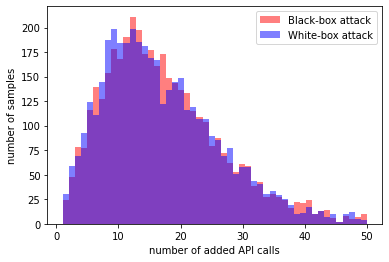
\includegraphics[width=0.5\textwidth]{attack-additions-histogram}
	\caption{Histogram of added API calls for successful attacks}
	\label{fig:added-calls}
\end{figure}

In comparison to \autocite[12]{DBLP:journals/corr/RosenbergSRE17} we observe 
that we achieved a similar attack effectiveness but our relative number of 
added API calls (attack overhead) was significantly worse. This is due to the 
circumstance that sequence length in our dataset (100) is significantly smaller 
than theirs (100,000 on average).

\subsection{Effects of adversarial training}
We observed that the adversarial training slightly decreased the model's 
performance on 
the test set to 95.7\% sensitivity and 93.5\% specificity. Fortunately, this 
performance is still pretty balanced despite the large class imbalance during 
training. Surprisingly, the adversarially trained model was very resistant to 
the attacks, at least within the maximum of 50 added API calls investigated 
here. More specifically, the white-box attack was successful for 0.7\% and the 
black-box attack was successful for 0.88\% of the samples. The baseline attack 
that picks the inserted API calls at random achieved a similar effectiveness of 
1.28\%. This significant decrease in effectiveness shows that the adversarial 
training made the model generally more robust against additions of API calls. 
Clearly, 
this effect was largest for the targeted attacks and basically degraded their 
performance to a random attack. However, this strong effect could also be an 
artifact of the original dataset only containing sequences of the same length 
and the model learning that any longer sequence is malicious. 
Nevertheless, we consider adversarial training to 
be an effective defense measure in the investigated setting.

\section{Conclusion}
\label{sec:conclusion}
All in all we showed that an LSTM malware classifier for Windows API call 
sequences can be effectively attacked by inserting API calls. Moreover, this 
effectiveness does not depend on the availability of the classifiers details 
such as gradients and is thus equally good in black-box and white-box settings. 
Additionally, we showed that adversarial training is a highly effective defense 
measure that basically degrades the investigated targeted attack to a random 
attack.

For future work it might be interesting to investigate datasets with longer and 
varying-length API call sequences, different model architectures or other 
defense methods. In 
addition to that a more realistic surrogate model training could be developed 
that takes the discreteness of API calls into account. It would be interesting 
to see whether that degrades the black-box attack effectiveness. Finally, to 
make this attack practically usable it should be explored which API calls with 
which parameters can be adversarially added to the malware without practical 
side-effects 
on the functionality and whether these additions are easily detectable and thus 
removable by a defender.

\printbibliography

\newpage
\appendix

\section{Appendix}

\counterwithin{figure}{section}
\counterwithin{table}{section}
\setcounter{figure}{0}
\setcounter{table}{0}

\begin{table}[H]
	\caption{LSTM architecture tuning results}
	\label{tab:architecture-tuning}
	\begin{tabular}{
			|>{\raggedright\arraybackslash}p{2.5cm}
			|>{\raggedright\arraybackslash}p{2.5cm}
			|>{\raggedleft\arraybackslash}p{1.8cm}|}
		\hline 
		\textbf{Fixed hyper-parameters} & \textbf{Investigated hyper-parameter} 
		& \textbf{Validation loss}\\
		\hline 
		\hline 
		$l_{LSTM} = 1$, $h_{LSTM} = 128$ & $pool = max$ & \textbf{0.005656} 
		\\
		\hline
		$l_{LSTM} = 1$, $h_{LSTM} = 128$ & $pool = avg$ & 0.016071 \\
		\hline
		\hline
		$pool = max$, $h_{LSTM} = 128$ & $l_{LSTM} = 1$ & \textbf{0.005656} 
		\\
		\hline
		$pool = max$, $h_{LSTM} = 128$ & $l_{LSTM} = 2$ & 0.006756 \\
		\hline
		$pool = max$, $h_{LSTM} = 128$ & $l_{LSTM} = 3$ & 0.021111 \\
		\hline
		\hline
		$pool = max$, $l_{LSTM} = 1$ & $h_{LSTM} = 64$ & 0.006979 \\
		\hline
		$pool = max$, $l_{LSTM} = 1$ & $h_{LSTM} = 128$ & \textbf{0.005656} 
		\\
		\hline
		$pool = max$, $l_{LSTM} = 1$ & $h_{LSTM} = 256$ & 0.006653 \\
		\hline
		$pool = max$, $l_{LSTM} = 1$ & $h_{LSTM} = 512$ & 0.007049 \\
		\hline
	\end{tabular} 
\end{table}

\end{document}
